\subsection{Reason}
В Reason добавлены следующие возможности:
\begin{itemize}

\item Можно использовать другой стиль стрелок («->» вместо «=>») в pattern matching.%, но в таком случае не работает {\it when} (одна из дополнительных функций).

\item Можно писать pattern matching в стиле \OCaml{}.%, но тогда после стрелки может идти только единичное выражение, а не их последовательность.%\footnote[1]{Однако эта проблема легко решается заключением последовательности в \{\}. }

\item Можно писать условие и тело цикла в стиле \OCaml{}.

\item Можно использовать разделитель <<;>> вместо <<,>> в объявлении record.

\item Можно объявлять модули в стиле \OCaml{}.

\item Можно писать {\it if} с {\it then}.

\item Добавлено ключевое слово {\it match}.% и теперь оно не может использоваться в качестве идентификатора.

\end{itemize}

Так же добавлены предупреждения (warning) для всех синтаксических конструкций перечисленных выше. И реализовано быстрое исправление кода (<<Quick fix>>) в OCaml-LSP, которое заменяет {\it match with} и {\it struct end} на подходящие языку Reason ключевые слова.
\begin{figure}[h]
%\fbox{
	\begin{subfigure}[t]{0.5\textwidth}
		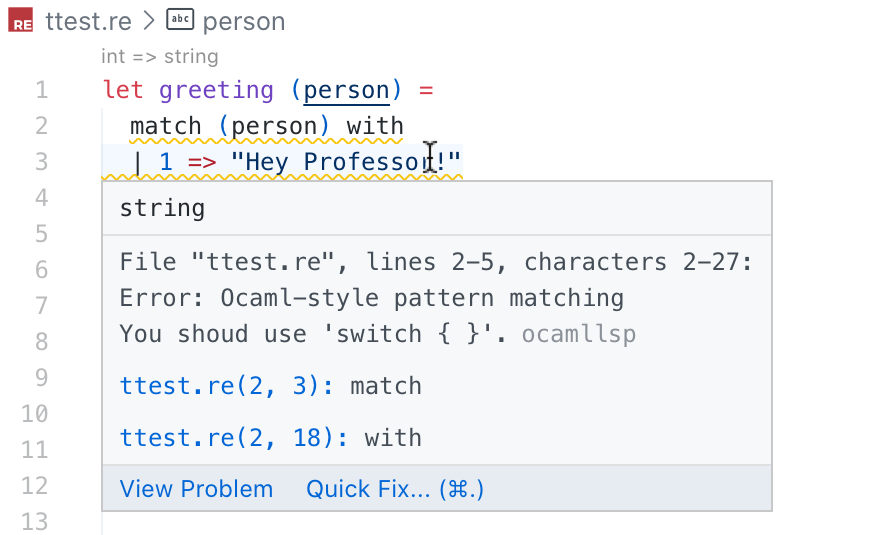
\includegraphics[width=\linewidth]{screenshots/05.png}
		\caption{IDE предупреждает о том, что pattern matching написан в стиле OCaml и \newline предлагает быстрое исправление.}
	\end{subfigure}
%}
	\begin{subfigure}[t]{0.5\textwidth}
		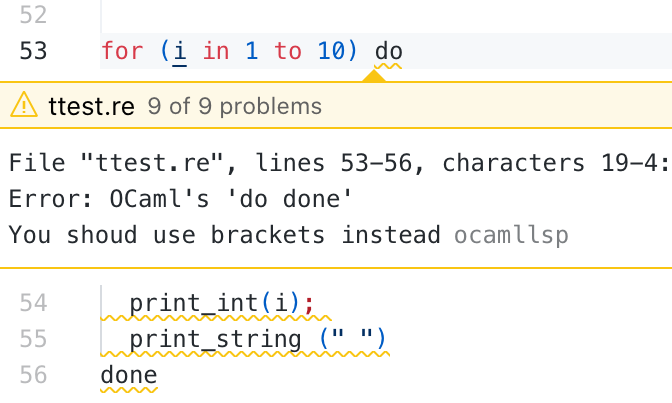
\includegraphics[width=\linewidth]{screenshots/06.png}
		\caption{IDE предупреждает о том, что цикл написан в стиле OCaml.}
	\end{subfigure}
\caption{Примеры предупреждений в коде Reason}
\end{figure}
\newpage
\subsection{OCaml}
Для симметричной задачи, для OCaml реализованы предупреждения в OCaml-LSP для следующих конструкций из Reason: определение модуля, pattern matching (при этом стрелки должны быть из OCaml), запятые в record. Для этих же конструкций реализованы соответствующие быстрые исправления в OCaml-LSP:
\begin{itemize}

\item Замена {\it \{ \}} на {\it struct end}.

\item Замена {\it switch \{ \}} на {\it match with}.

\item Замена всех <<,>> на <<;>> в объявлении record.

\end{itemize}

\begin{figure}[h]
	\begin{subfigure}[t]{0.5\textwidth}
		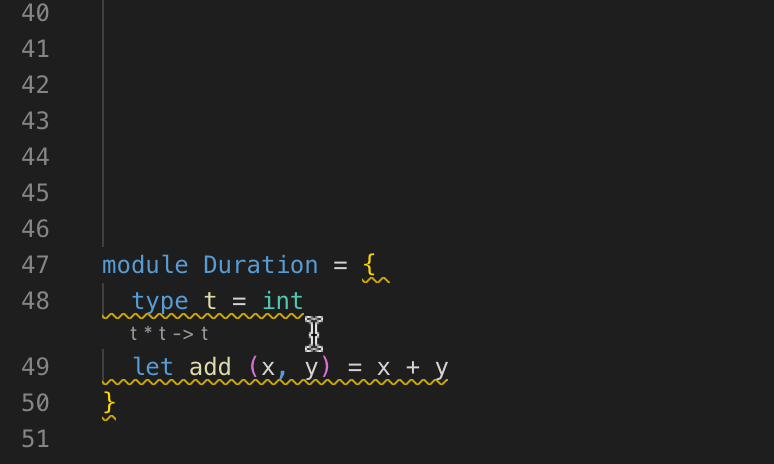
\includegraphics[width=\linewidth]{screenshots/01.png}
		\caption{Неверно написанная конструкция выделяется цветной волной.}
	\end{subfigure}
	\begin{subfigure}[t]{0.5\textwidth}
		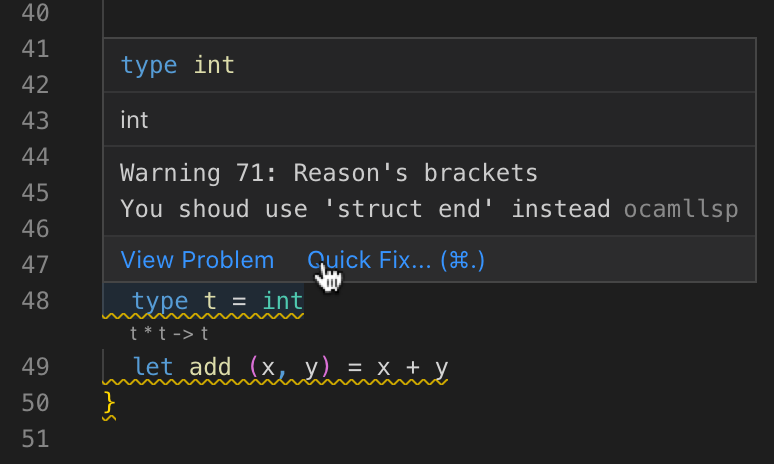
\includegraphics[width=\linewidth]{screenshots/02.png}
		\caption{IDE предлагает <<Quick fix>>.}
	\end{subfigure}
	\newline
	\begin{subfigure}{0.5\textwidth}
		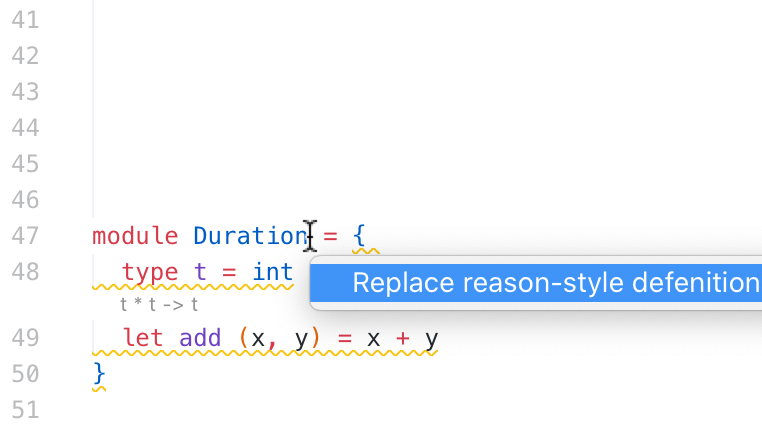
\includegraphics[width=\linewidth]{screenshots/03.png}
		\caption{Кнопка запускающая замену.}
	\end{subfigure}
	\begin{subfigure}{0.5\textwidth}
		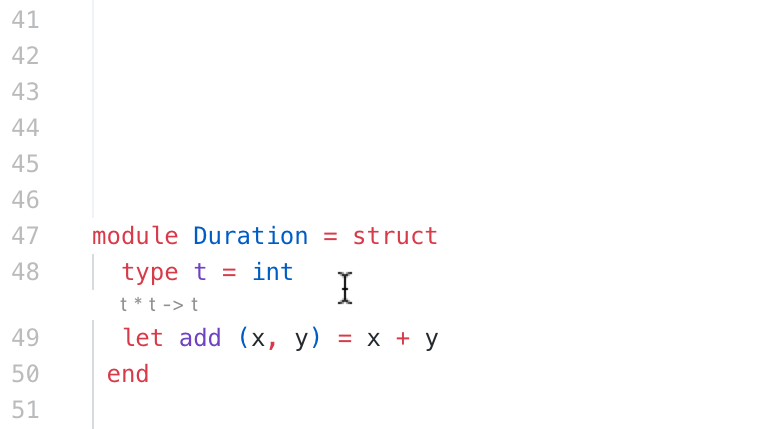
\includegraphics[width=\linewidth]{screenshots/04.png}
		\caption{Исправленная конструкция.}
	\end{subfigure}
\caption{Исправление кода OCaml}
\end{figure}

\newpage

\subsection{Архитектура}
\begin{figure}[h]
	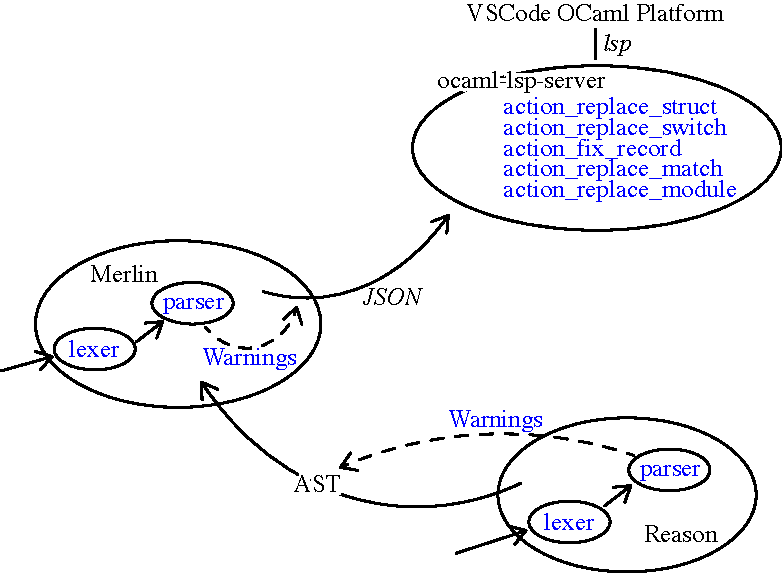
\includegraphics[width=\linewidth]{graph.pdf}
\caption{Архитектура расширения. Стрелки обозначают передачу данных. Курсивом выделены протоколы. Синим цветом выделены части, которые подверглись изменениям, зеленым~--- новые модули.}
\end{figure}
Поддержка OCaml в Reason реализована через новые синтаксические правила для парсера. Для этих правил так же созданы предупреждения (warnings), как новый тип reason\_warning, по примеру существующего в Reason типа reason\_error. Во время работы парсера предупреждения выкидываются из него и собираются. Далее они, с помощью добавленной функции warning\_attribute, превращаются в атрибуты AST и вместе с ним передаются в merlin, откуда идут в ocaml-lsp и в итоге в IDE. Необходимая поддержка атрибутов reason.warning добавлена на стороне merlin.

Поддержка Reason в OCaml реализована через новые правила для парсера и расширение стандартного списка предупреждений OCaml.

Функции исправления кода в ocaml-lsp как для Reason, так и для OCaml созданы по примеру action\_add\_rec\footnote{ \url{https://github.com/ocaml/ocaml-lsp/blob/master/ocaml-lsp-server/src/code_actions/action_add_rec.ml} (accessed: 24.08.2022) }. Action\_add\_rec~--- это code\-Action, добавляющий слово {\it rec} перед рекурсивной функцией, если его еще не было. CodeAction, являющийся частью спецификации протокола lsp, представляет собой изменение, которое может быть выполнено в коде, например для рефакторинга кода.

Стоит заметить, что для Reason реализована поддержка второго языка как при {\it компиляции}, так и в {\it IDE}, тогда как у OCaml только для {\it IDE}. Такая ситуация возникла из-за того, что у Reason одна кодовая база для парсера, компилятора и reason-merlin, в отличии от OCaml, где два разных репозитория для компилятора и Merlin. В нашем случае частичная поддержка Reason была добавлена только в Merlin.

\subsection{Установка}
Необходимая для ocaml-lsp версия OCaml~--- 4.13.1/4.13. Reason совместим с версиями 4.13.1/4.13/4.12.1/4.12. Так же понадобится opam. Все необходимые пакеты устанавиваются следующими командами:

% ":" not italic, i don't know
\lstset{emph={https}, emphstyle={\itshape \small} }
\lstset{basicstyle=\ttfamily}
\begin{example}
\begin{lstlisting}[frame=single,
language=C,
% fix stupid bug with bad "-" in copying from pdf
literate={-}{-}1
]
opam pin add reason https://github.com/pereb4ik/reason.git
opam pin add ocaml-lsp-server https://github.com/pereb4ik/ocaml-lsp.git
\end{lstlisting}
\caption{Команды установки Reason и ocaml-lsp}
\end{example}
Для тестирования функций IDE таких, как умная замена кода <<Quick fix>>, понадобится Visual Studio Code (хотя ocaml-lsp можно использовать с другими редакторами) с расширением OCaml Platform от OCaml Labs.

Результаты проделанной работы можно наблюдать в соответсвующих репозиториях. Ссылки на списки коммитов Reason\footnote{ \url{https://github.com/pereb4ik/reason/commits?author=pereb4ik} (accessed: 8.08.2022) },
OCaml-LSP\footnote{ \url{https://github.com/pereb4ik/ocaml-lsp/commits?author=pereb4ik} (accessed: 8.08.2022) },
merlin\footnote{ \url{https://github.com/pereb4ik/merlin/commits/lsp?author=pereb4ik} (accessed: 8.08.2022) }.